\documentclass{article}

\usepackage{graphicx}
\usepackage{tikz}
\usepackage{tikzsymbols}
\usetikzlibrary{calc,patterns,shapes.geometric}
\pagestyle{empty}
\usepackage[margin=0pt]{geometry}
\geometry{papersize={14in,12in}}

\def\centerarc[#1](#2)(#3:#4:#5){\draw[#1] ($(#2)+({#5*cos(#3)},{#5*sin(#3)})$) arc (#3:#4:#5);}

\begin{document}
	\begin{figure}
		\centering
		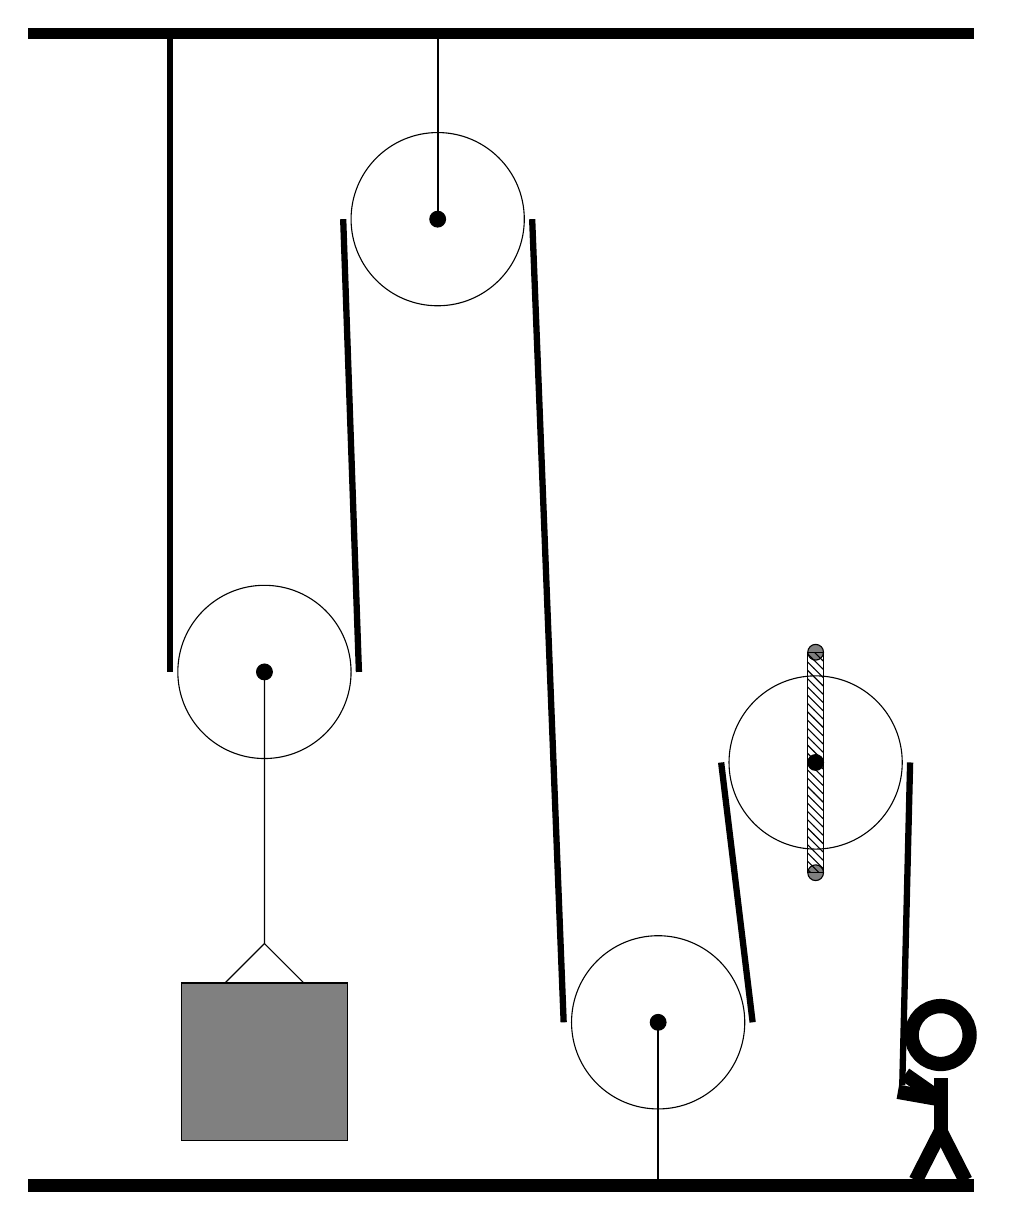
\begin{tikzpicture}
			%%%%% START %%%%%
			\draw[fill=black] (-2, 11.5) rectangle (10, 11.625);
			
			\draw (1, 3.45) circle (1.1);
			\draw[fill=black] (1, 3.45) circle (0.1);
			
			\draw (3.2, 9.2) circle (1.1);
			\draw[fill=black] (3.2, 9.2) circle (0.1);
			\draw[thick] (3.2, 9.2) -- (3.2, 11.5);
			
			\draw (6, -1) circle (1.1);
			\draw[fill=black] (6, -1) circle (0.1);
			\draw[thick] (6, -1) -- (6, -3);
			
			\draw[fill=white](8, 2.3) circle (1.1);
			\draw[fill=black] (8, 2.3) circle (0.1);
			\draw[fill=black!50] (8, 3.7) circle (0.1);
			\draw[fill=black!50] (8, 0.9) circle (0.1);
			\draw[pattern=north west lines, pattern color=black] (7.9, 3.7) rectangle (8.1, 0.9);
			
			\draw (1, 3.45) -- (1, 0.0) -- (0.5, -0.5);
			\draw (1, 0.0) -- (1.5, -0.5);
			\draw[fill=black!50] (-0.05, -0.5) rectangle (2.05, -2.5);
			
			\draw[line width=0.8mm] (-0.2, 11.5) -- (-0.2, 3.45);
			\centerarc[line width=0.8mm](1, 3.45)(180:360:1.2000000000000002);
			\draw[line width=0.8mm](2.2, 3.45) -- (2.0, 9.2);
			\centerarc[line width=0.8mm](3.2, 9.2)(0:180:1.2000000000000002);
			\draw[line width=0.8mm](4.4, 9.2) -- (4.8, -1);
			\centerarc[line width=0.8mm](6, -1)(180:360:1.2000000000000002);
			\draw[line width=0.8mm](7.2, -1) -- (6.8, 2.3);
			\centerarc[line width=0.8mm](8, 2.3)(0:180:1.2000000000000002);
			\draw[line width=0.8mm](9.2, 2.3) -- (9.1, -1.8);
			
			\node at (9.5, -1.9) {\Strichmaxerl[10][-35][170]};
			
			\draw[fill=black] (-2, -3) rectangle (10, -3.15);
			%%%%% END %%%%%
		\end{tikzpicture}
	\end{figure}	
\end{document}